% 2010 年四川卷理科第 11 题：球 O、直径 AB⊥平面 α 于 B，正三角形 BCD 在 α 内，
%   线段 AC、AD 与球面交于 M、N。
% 来源 PDF：普通高考/2010/2010四川理.pdf，SHA-256 499425696359cfc2cf4418254bdaa1a37487b3dbaa072ff3c7cbe18dbabe73dc。
% 原页：第 1 页（A3 三栏）第 2 栏中部，书页码 631。
% 重绘依据：球画成圆 + 赤道椭圆（后半虚线、前半实线）；平面 α 画成平行四边形，球与之相切于 B，
%   平面远边被球遮挡处留白；△BCD 整个落在平行四边形内（BC、CD 实线，BD 被球遮挡用虚线）；
%   AC、AD 在球内的部分（A—M、A—N）与直径 AB 同样画虚线，球外部分（M—C、N—D）画实线。
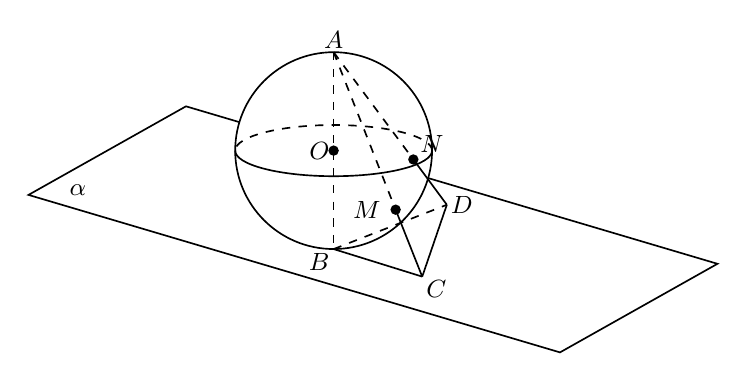
\begin{tikzpicture}[scale=1.25, semithick, every node/.style={inner sep=1.2pt, font=\small}]
  % ===== 平面 α（平行四边形，近边在三角形下方）
  \draw (-3.10,-0.45) -- (2.30,-2.05) -- (3.90,-1.15) -- (-1.50,0.45) -- cycle;
  \node at (-2.60,-0.40) {$\alpha$};

  % ===== 球面（白色填充遮挡后画的平面远边）
  \fill[white] (0,0) circle (1.00);
  \draw (0,0) circle (1.00);
  % 赤道：后半（上）虚线、前半（下）实线
  \draw[dashed] (1,0) arc (0:180:1.00 and 0.26);
  \draw (-1,0) arc (180:360:1.00 and 0.26);

  % ===== 直径 AB（球内，虚线）
  \coordinate (A) at (0,1.00);
  \coordinate (B) at (0,-1.00);
  \coordinate (O) at (0,0);
  \draw[dashed] (A) -- (B);

  % ===== △BCD（平面 α 内）
  \coordinate (C) at (0.90,-1.28);
  \coordinate (D) at (1.15,-0.55);
  % M、N 取在线段 AC、AD 上，距 A 约 70%
  \coordinate (M) at (0.63,-0.60);
  \coordinate (N) at (0.81,-0.09);
  \draw (B) -- (C);
  \draw (C) -- (D);
  \draw[dashed] (B) -- (D);

  % ===== AC、AD 在球内部分虚线、球外部分实线
  \draw[dashed] (A) -- (M);
  \draw[dashed] (A) -- (N);
  \draw (M) -- (C);
  \draw (N) -- (D);

  % ===== 点与标注
  \fill (O) circle (1.5pt);
  \fill (M) circle (1.5pt);
  \fill (N) circle (1.5pt);
  \node[above] at (A) {$A$};
  \node[left] at (O) {$O$};
  \node[below left] at (B) {$B$};
  \node[below right] at (C) {$C$};
  \node[right] at (D) {$D$};
  \node[left=4pt] at (M) {$M$};
  \node[above right=1pt] at (N) {$N$};
\end{tikzpicture}
